\part{Calculs acoustiques}
	\chapter*{Introduction}
	\addcontentsline{toc}{chapter}{Introduction}
Dans cette partie, nous allons traiter d'acoustique, d'algorithmes et de mathématiques. Chacune de ces disciplines permettra de répondre aux questions suivantes : Pourquoi ? Quoi ? Comment ? Voyons donc ces problématiques une par une.\\

\textit{\textbf{Pourquoi ?}} L'objectif de notre projet, maintenant que nous disposons d'une maquette virtuelle du théâtre d'Orange, est d'en étudier l'acoustique. Nous souhaitons pouvoir simuler, écouter et étudier le son qui était perçu dans ce lieu il y a deux mille ans. Outre le fait d'acquérir ces données, nous avons vu que les restitution de certaines parties du théâtre était plus ou moins hypothétiques. Nous pourrons comparer ces différentes tentatives de restitution et en mesurer l'impact visuel mais également auditif. Les rares écrits antiques et les récentes études acoustiques sous-entendent que les Romains, et avant eux les Grecs, se basaient énormément sur la physique des matériaux et la géométrie des monuments pour optimisé la propagation sonore. Nous allons donc tenter d'apporter notre pierre à l'édifice au sujet de cette question.

\textit{\textbf{Quoi ?}} Cet objectif nous a amené à développer un outil de calcul numérique répondant à des problématiques précises. Il complète la première partie de ce projet en s'interfaçant directement au logiciel Blender. Ainsi nous pourrons étudier la maquette virtuelle du théâtre d'Orange simplement. Néanmoins, il est important de noter que cet outil est générique. Il pourra donc agir sur différents type de problèmes. Dans cette partie nous le décrirons d'ailleurs d'un point de vu algoritmique dans son contexte général.

\textit{\textbf{Comment ?}} Tout code informatique présente une part de calcul, et qui dit calcul, sous-entend mathématiques. Ainsi, nous verrons les méthodes et astuces mathématiques qui ont permis de développer ce programme. Nous détaillerons les notions de lancer de rayons statistique, de sources images spatialisée et de réponse impulsionnelle. Aussi, nous verrons comment sont optimisées les performances par un procédé de "\textit{divide and conquer}" utilisant des octree. Un chapitre est également consacrer à la validation de l'algorithme en utilisant notamment des méthodes analytiques.\\

Pour débuter, nous ferons un tour d'horizon de la physique de l'acoustique et plus concrètement dans le cas qui nous concerne, de l'acoustique de salle. Nous présenterons les différentes méthodes permettant d'étudier les lois acoustiques et présenterons leurs limites. Nous détaillerons alors les principes physiques utilisés pour notre algorithme avant de passer à la présentation de son architecture et à sa validation.


\chapter{Acoustique de salle}
		\citationChap{
			La musique, c'est 50\% d'un film.}
			{Georges Lucas}
		\minitoc
		\newpage
		
\section{Introduction à l'acoustique de salle}
L'acoustique de salle est une discipline à part entière qui consiste principalement à étudier la réverbération d'une pièce soumis à une onde sonore. Le principe de cette étude est le suivant : Il s'agit en général de placer une source sonore à l'intérieur d'une salle, fermée ou non, et de la faire rayonner dans toutes les directions. L'onde se propage alors jusqu'aux parois et subit un phénomène de diffusion. Il s'agit en réalité d'une combinaison de trois phénomènes : la réflexion, la réfraction et la diffraction. Par réfraction on entend la notion d'absorption suivant les lois de Descartes sur la propagation entre deux milieux (\cite{jouhaneau}). La diffraction quant à elle opère lorsque la longueur d'onde est proche de la taille de l'obstacle. En se plaçant en un point à l'intérieur de la salle, on pourra alors recevoir un signal sonore comme étant la somme d'un champ direct et d’un champ réverbéré. Le son direct provient directement de la source sans n'avoir touché aucune surface. Le son réverbéré se distingue en deux catégories : les premières réflexions dont l'ensemble forment la texture du son et le champ diffus qui peut être assimilé à une somme infinie d'ondes se propageant dans toutes les directions. 
On comprend alors que les principaux facteurs qui vont influer sur l'acoustique perçue dans une salle sont : la source sonore, le milieu de propagation et la nature des parois et des obstacles.

\begin{figureth}
	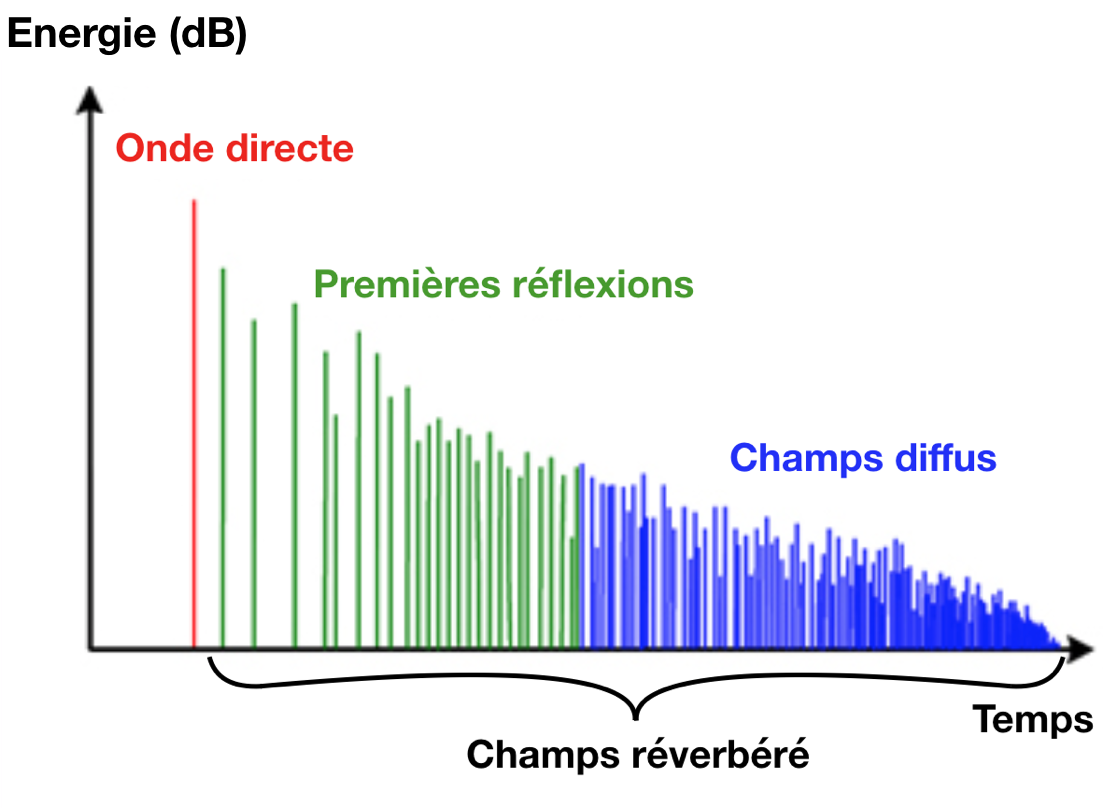
\includegraphics[width=\linewidth]{images/RIR_schematique}
	\caption{Réponse schématique temporelle d'une impulsion sonore dans une salle}
	\label{RIR_schematique}
\end{figureth}

La figure \ref{RIR_schematique}, présentant schématiquement une réponse impulsionnelle, montre que l'information perçue est une succession d'ondes sonore arrivant décalées dans le temps. Si l'écart entre ces ondes est long, alors d'auditeur pourra les différencier et entendra le phénomène d'écho. Au contraire, si l'écart est suffisamment restreint et que les ondes sont mélangées au moment d'arriver à l'auditeur, alors celui-ci n'entendra qu'un son prolongé dont l'intensité diminue. Il s'agit de la réverbération (\cite{sabine}). La théorie de Sabine, couramment employée en acoustique des salles, suppose que l’énergie sonore et le temps de réverbération sont uniformes en tout point de la salle. Ces considérations permettent d'exprimer ces deux valeurs l'une par rapport à l'autre comme par exemple dans la formule de Sabine : 

\begin{equation}
   	T = \frac{k.V}{A}
\end{equation}

Avec : \\
$k \approx 0,163$ \\
$V$ : le volume de la salle\\
et
\begin{equation}
   	A = \sum_{i=1}^N S_{i}\alpha_{i} + 4mV
\end{equation}
où : \\
$\alpha$ est le coefficient d'absorption \\
$m$ est l'amortissement du milieu (par exemple l'air) \\
$S_{i}$ est la surface de la i\up{e} \\
$N$ est le nombre de paroi total \\

Malheureusement, cette hypothèse dite de champ diffus n’est plus vérifiée en pratique, dès lors que la forme du milieu de propagation n’est plus homogène et que l’absorption acoustique devient importante et non uniforme. De plus, cette théorie s’applique mal aux géométries présentant des ouvertures et, en particulier, dans le théâtre d'Orange. \cite{picaut}.

\section{Méthodes de calcul acoustique} 

	\subsection{Méthode de résolution exacte}
%La méthode des éléments finis de frontère consiste quant a elle a mailler le domaine d'étude par des petits éléments linéiques (2D) ou surfaciques (3D). Sur chaque sous-domaine ainsi défini, la pression est calculée par une interpolation des valeurs en des points choisis arbitrairement sur le sous-domaine et appeles points nodaux. Le problème se ramène alors a la résolution d'un système d'équations aux valeurs propres. L'avantage de la méthode des eléments finis est qu'elle consiste finalement a inverser une matrice creuse.
%	
	
	\subsection{Méthode de tracé de rayon}
	très démocratisée, a donné naissance à de
nombreux logiciels commerciaux de prévision du champ sonore, aussi bien en acoustique des salles
qu’en milieu extérieur. Cette approche, également géométrique, suppose que l’énergie sonore est
distribuée à un certain nombre de rayons rectilignes émis à partir d’une source sonore et déviés de
manière spéculaire lors de leur rencontre avec les parois du milieu de propagation. Le calcul de
l’énergie sonore au niveau d’un volume récepteur est réalisé par comptage du nombre de rayons qui
le traversent. Le problème majeur réside dans la définition de la taille de ce volume, le plus souvent
une sphère. En effet, il doit être représentatif d’un récepteur réel, mais doit également permettre de
comptabiliser suffisamment de rayons sonores pour déterminer le niveau d’énergie de manière
précise, ce qui en pratique nécessite de tirer un grand nombre de rayons sonores, et ce d’autant plus
que le milieu de propagation est de forme complexe et constitué de volumes couplés. \cite{picaut}.
	
	\subsection{Méthode des sources-image}
	Elle est fondée sur la construction de sources virtuelles,
images de sources réelles, simulant l’effet des réflexions successives de l’énergie sonore sur les parois
de l’enceinte. La contribution énergétique de chaque source-image en un point donné est celle
habituellement rencontrée dans le cas de la propagation en champ libre, pondérée par le coefficient
d’absorption des parois considérées. Cette approche, principalement numérique, est néanmoins
réductrice dans la mesure où les réflexions sur les parois du domaine sont traitées intégralement de
manière spéculaire (angle de réflexion égal à l’angle d’incidence), alors que de nombreux auteurs ont
montré l’importance des effets des réflexions diffuses dans le calcul du champ sonore [Hodgson,
1991] et dans les procédures liées à l’auralisation [Torres et al., 2001]. \cite{picaut}.
	
	\subsection{Méthode de lancé de particules}
chaque rayon sonore est porteur d’une intensité dont
l’amplitude décroît proportionnellement avec le carré de la distance de propagation, simulant ainsi
le rayonnement acoustique d’une source sphérique (dispersion géométrique). À l’inverse, dans le
concept des particules sonores, chaque particule est porteuse d’une énergie constante.

%Par exemple, au contact avec
%une paroi de coefficient d’absorption α, l’intensité du rayon après réflexion sera pondérée par le
%coefficient (1–α). Dans l’approche « particules sonores », ces phénomènes physiques sont considérés
%de manière probabiliste. Au contact avec une paroi de coefficient d’absorption α, la particule aura
%une probabilité (1–α) d’être réfléchie, et une probabilité α d’être absorbée. Dans ce dernier cas, elle
%disparaît du domaine de propagation.

Dans l’approche particulaire, ces réflexions
diffuses sont considérées de manière probabiliste, l’angle de réflexion pouvant être choisi suivant
une loi quelconque de réflexion arbitraire.
Dans l’approche
particulaire, les objets diffusants peuvent être considérés de manière statistique, sans aucune autre
connaissance que leur distribution spatiale et leur forme moyenne, ce qui réduit de manière
significative les coûts en termes de calcul et de définition du domaine d’étude. \cite{picaut}.
	
	\subsection{Statistique}
\section{Méthode couplée}
pour être complet, il faut également signaler que la plupart de ces approches,
comme celles fondées sur les sources images et le tracé de rayons sonores, prennent difficilement en
compte les effets météorologiques tels que le vent, les gradients de célérité du son et la turbulence
atmosphérique, pourtant très importants en milieu ouvert [Piercy, 1977 ; Embleton, 1996], \cite{picaut}.

		
\chapter{Logiciel développé}
	\citationChap{
	Quand on aime on ne compte pas... \\
	Ça tombe bien, je suis mauvaise en calcul !
	}{Sophie Lesellier}
	\minitoc
	\newpage
	
\section{Introduction}
Rappel des problématiques, conditions choisies (source omni, parois non diffusante)
\section{Lecture de maillage}
\section{Calcul de rayon}
\section{Calcul de sources-images}
\section{Génération de réponse impulsionnel}
\section{Méthode d'octree}
\section{Vue d'ensemble}
Add-on blender, traitement du signal, etc

\chapter{Validation}
	\citationChap{
	L'observateur modifie ce qu'il observe. Certains événements ne se produisent que parce qu'ils sont observés. Sans personne pour les voir ils n'existeraient pas. 
	}{Bernard Werber}
	\minitoc
	\newpage
	\section{Introduction}
	Rappel cahier des charges
	\section{Comparaison aux cas test}
		\subsection{Salle rectangulaire}
		\subsection{Salle sphèrique}
	\section{Analyse de complexité}
	
\chapter*{Conclusion}
\addcontentsline{toc}{chapter}{Conclusion}
	\newpage
	
% Biblio
 \bibliographystyle{francaissc}
 \bibliography{Part2/Biblio}
\addcontentsline{toc}{chapter}{Références}
